Applying information theoretical algorithms on a high density EEG dataset is the main focus of this thesis. The EEG dataset is provided by the lab of computational neuroscience of KU Leuven. In order to perform an analysis of a dataset, it is important to understand what kind of data we are dealing with.

This chapter discusses the experiment used to generate the dataset. The experiment and the reasons behind the experiment are introduced. Afterward the actual experiment is discussed. This starts with the an explanation of the EEG experiment itself and the paradigm. Afterwards the source localization is discussed. Finally, the final structure of the data is brievely discussed.

\section{Introduction}

The experiment resolves around the human brain's representation of semantic categories. By using high density EEG recordings, the semantic processing of words within the human brain was captured. Within the literature, there are several different theories and concepts that explain the representation of semantic categories within the human brain. The human brain is a complicated organ with many different cortical areas. Each theory focusses on different cortical areas and explain how they are involved with the representation of semantic categories. These theories have been further developed with the aid of different neuroimaging experiments. 

One of the most prominant theories of semantic word processing is the grounded cognition model. The model is also called the embodied cognition model. This model explains that semantic knowledge is kept within high-level perception and motor representation systems in the brain. 

This means that a word is comprehended based on modality-specific neural systems. In other words, elements such as visual and auditory features are used to define words. 

\todo{to be rewrited}

Examples in favour of the embodied cognition theorem are fMRI studies showing that animate objects cluster in the more lateral aspect of the fusiform gyrus, whereas activations associated with inanimate or man-made objects cluster in the more medial aspect of the fusiform gyrus (Chao et al., 2015), additionally there are certain category mappings based on specific shape, such as "face" and "body" patches (Tsao et al., 2008). There is also support coming from lesion studies where damage to the brain's modal system creates category-specific deficits, disproportionately preserving categories such as animals, foods, or artefacts (Barsalou et al., 2003; Caramazza and Mahon, 2003). To explain these deficits according to the grounded cognition model, they claim natural objects such as animal, fruits and vegetables etc, are distinguished primarily from their visual semantic properties, while man-made items such as tools and vehicles are vehicles are distinguished primarily by their function, as evidenced by fMRI and PET imaging studies (Devlin et al., 2002).

The grounded cognition model, and its extension into the hubs and spoke model as an attempt to explain the ability of between category and within category differentiation despite overlapping modality-specific features (Ralph and Ralph, 2013)  can be criticized from several aspects. First of all, modality-specific features of a concept are much less variant between different subjects when shown as a clear visual stimuli (image). However, when stimuli are conceptual in nature (such as words presented in written or spoken form) the perceptual and motor-sensory function they evoke are much more difficult to control, as the experience designated to specific entities is subject-dependent to a larger degree (Kemmerer, 2015). Secondly, and especially relevant for our study is that the grounded cognition model only explains features that are rooted in physical experience with a concept. However, abstract concepts, such as "democracy" or concepts related to emotions are not explained by this theory, even though the vast majority of human language actually constitutes abstract concepts.

The difference in the processing of abstract and concrete words, has been tackled by some theories, the main ones being the dual coding theorem, and the context availability theorem (Kounios and Holcomb, 1994; Wang et al., 2010). In the dual coding theorem, the claim is that two separate systems reside in the brain, a nonverbal "imagery" system the verbal ("linguistic") system which implements the modality-specific aspects of a concepts (not unlike the grounded cognition model), and a purely verbal "linguistic" system which is more involved in the abstract form of language. According to the context availability theorem, the processing of concrete and abstract words never happens in isolation, but is aided by the context by which the word can be understood. Since the context of concrete words are constrained by their physical referents, understanding them will again involve modality-specific brain systems as defined in the grounded cognition model. In the case of abstract concepts however, context is more variable and experience dependent. 

Both theories have neither been proved nor disproved by scientific literature, and research is still in progress. One most vital limitation of all aforementioned theories is that they have been predominantly studied using functional neuroimaging techniques such as fMRI and PET, which is limited in terms of temporal resolution (Bookheimer, 2002), even though visual word recognition is a complex dynamic process that involves several cognitive stages happening on millisecond scale, such as visual encoding, lexical activation, and semantic presentation (Bentin, 1999). Whether temporal activation of these stages are sequential or partially parallel, interactive processes is not known, however it is clear that heamodynamic measures cannot follow the progress of activation of different areas, which result in a different pattern of activity for each word (Bentin, 1999; Salmelin et al., 1998). On the other hand studies involving lesions and electrical stimulations do no give a good spatial overview on the large-scale networks involved.

By virtue of its excellent temporal resolution, the EEG technique has been hailed to probe the brain's detailed processing of objects and words. Studies using EEG/ERP recordings have successfully distinguished differences in word categories on different stages of semantic processing, starting from difference in word length and word frequency revealed earlier in the time course between 100 and 200 ms (Hauk et al., 2006), to distinction in processing of semantic categories, such as abstract concepts versus concrete concepts (Bentin, 1999), animals verus tools (Simanova et al., 2010) and more generally natural objects versus artefacts (Kiefer, 2001) which occurs later in the time course as revealed by the N400 potential.

The main drawback of the EEG is it's relatively low spatial resolution, and in this way falls short in detecting differences in cortical network activation. For example, it is possible that different aspects of semantic activity and language comprehension are associated with different negativities during the same time epoch, explaining the differences in the N400 scalp distribution as being caused by different neural generators (Bentin, 1999). Therefore, spatial resolution is equally vital to obtain a complete picture of what is happening.

In this study, using high density EEG recordings, we were able to capture the fast dynamics involved in semantic processing as we localized the neural activity on the cortex with an accuracy in the range of millimetres and milliseconds. This will provide us with a unique opportunity to investigate the spreading of activity during the processing of semantic features.

\section{Materials and methods}

The experiment was done in a sound-attenuated, darkened room with a constant temperature of 20 degrees, sitting in front of an LCD screen at a distance of about 70cm.

EEG data is recorded using 128 active Ag/AgCl electrodes (SynampsRT, Compumedics, France), according to the international 10-20 system. Two of these electrodes serve as ground (AFz) and reference (FCz). The EEG signal is recorded at a 2 KHz sampling rate and downsampled to 500 Hz. All electrodes are mounted in an electrode cap that is placed on the subject's head (Easycap, Germany). 

\section{Experimental Paradigm}

In order to ensure that our subjects are involved in semantic processing and not just in lexical access (as would be the case with a lexical decision task), we choose a categorization paradigm consisting of 600 Dutch words (only nouns) taken from the database of concreteness ratings for 30,000 Dutch words (Brysbaert et al., 2014). Abstract words were selected based on having a concreteness rating of maximum 2.5, and concrete words had to have minimum of 3.5. Concreteness ratings of abstract and concrete words were found to be statistically different using t-test. Word length and word frequency for both groups of words were controlled, no significant difference  where found between. Word length and frequency were deduced from the Dutch CLEARPOND software (Marian et al., 2012). Additionally, words were pseudo randomly organized in such a way that no two consecutive words would have a high forward association, and forward associations were controlled for all consecutive words. Forward associations were taken from the Dutch free association network created by De Deyne et al (De Deyne et al., 2008). 

In each trial, a single white word is shown on a black screen for 300ms, followed by a question mark that lasts for 1 second. Prior to each trial, a fixation cross appeared on the screen, cueing subjects to focus in the middle part of the screen. Participants are asked to press the mouse button, on the moment they see the question mark, only if the word they are shown is a colour. The colour category is therefore used a non-target (called "filler") and will not be included in the results. After pressing a mouse button they received visual feedback on the button press ("kleur!" (colour) if pressed correctly, and "fout!" (wrong) otherwise). 

\begin{figure}[!htb]
\caption{Binning representation.}
\label{entropy}
    \centering
    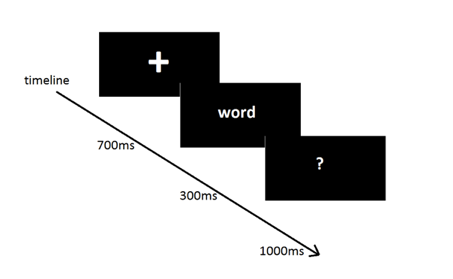
\includegraphics[width=\textwidth]{fig/experiment}
\end{figure}

\section{Source localization}
For our source reconstruction analysis we used the Brainstorm toolbox (Tadel et al., 2011), freely available under the GNU general public license. The default anatomy was based on the ICBM-152 template. For the forward model we used OpenMEEG BEM (Gramfort et al., 2010), in which case the cortex was divided into 15,000 dipoles. Noise covariance and data covariance matrices were obtained by merging the matrices calculated from the baseline of all selected trials. As our inverse modelling method, we used sLORETA (Pascual-Marqui, 2002) as it has shown to yield zero localization error in the absence of noise and to support the reconstruction of multiple sources. Source orientation was constrained to be orthogonal to the cortical surface. The signal-to-noise ratio (SNR) was set to the default value suggested by the Brainstorm Toolbox (SNR = 3). In addition, sulci are not taken into consideration during our analysis, as accurate source localization in these regions is implausible, as stipulated in Brainstorm's documentation.

In order to verify the correctness of our procedure, we attempted to reproduce the results using different source localization algorithms, as is recommended by (Mahjoory et al., 2017). We did not pursue the entire statistical procedure, however, we did analyze our initial results by taking the average over all trials regardless of semantic features, using the four methods available in the brainstorm toolbox: wMNE, dSPM, sLORETA, and unconstrained sLORETA. Manual inspection of the results with these methods revealed that the spatial distributions are similar over time albeit with different degrees of spatial smoothing.

\section{ROI selection}
 
(TODO)